\chapter{Implementação}

\section{Biblioteca}

Para o cálculo do \ac{HMAC} há uma classe respons\'{a}vel pela gera\c{c}\~{a}o das chaves (\ac{HMAC}KeyGenerator), uma pelo cálculo do \ac{HMAC} (\ac{HMAC}Calculator), al\'{e}m das classes que representam a chave para ser utilizada 
no cálculo do \ac{HMAC} (\ac{HMAC}Key) e o \ac{HMAC} em si (\ac{HMAC}).
A partir de uma chave \ac{HMAC} \'{e} poss\'{i}vel inicializar o \ac{HMAC}Calculator. Nele, \'{e} poss\'{i}vel adicionar dados para o calculo do \ac{HMAC} e finalizar a opera\c{c}\~{a}o.
 O trecho de código \ref{fonte:calculoHMAC} demonstra como é feito o cálculo do \ac{HMAC} de uma mensagem qualquer.

\lstset{language=JAVA,
	basicstyle=\small,
        breaklines=true,
        numbersep=5pt,
        xleftmargin=.35in,
        xrightmargin=.35in}
\begin{lstlisting}[label=fonte:calculoHMAC, caption=Exemplo do cálculo do HMAC]
    HMacKey key = HMacKey::generate("SHA1");
    HMACCalculator hmacCalc = new HMACCalculator(key);
    hmacCalc.update("mensagem");
    HMAC hmac = hmacCalc.doFinal();
\end{lstlisting}

Para o hist\'{o}rico cifrado, tem-se a classe respons\'{a}vel pelo cálculo (EncryptedHistoryCalculator) e a classe que representa o hist\'{o}rico cifrado (EncryptedHistory).
 Para iniciar o cálculo do hist\'{o}rico, é necessário uma chave sim\'{e}trica (SymmetricKey), que pode ser gerada de forma semelhante à chave utilizada pelo \ac{HMAC}, pela classe SymmetricKeyGenerator
 . Para o cálculo do hist\'{o}rico, é necessário fornecer uma lista de \ac{HMAC}s e uma chave sim\'{e}trica, coforme ilustrado no trecho de código \ref{fonte:calculo-historico}.

\lstset{language=JAVA,
	basicstyle=\small,
        breaklines=true,
        numbersep=5pt,
        xleftmargin=.35in,
        xrightmargin=.35in}
\begin{lstlisting}[label=fonte:calculo-historico, caption=Exemplo do cálculo do HMAC]
public EncryptedHistory generate(List<HMac> hMacs) throws SymmetricCipherException, EncryptionException {
	List<HMac> h = new ArrayList<HMac>();
	for(HMac hMac : hMacs) h.add(hMac.clone());
	byte[] xor = h.get(0).getBytes();	
	for (int i = 1; i < h.size(); i ++) {
		byte[] hmac = h.get(i).getBytes();
		for (int j = 0; j < hmac.length; j++)
			xor[j] = (byte) (xor[j] ^ hmac[j]);
	}
	byte[] result = cipher.doFinal(xor);
	return new EncryptedHistory(result);
}
\end{lstlisting}

\subsection{Provider}

\TODO{Um nome melhor para essa subseção, ja que vai ter uma seção para a implementação do provider. (Provedor de serviços?)}

A classe SecurityService possibilita efetuar diretamente o cálculo de \ac{HMAC}, Hist\'{o}rico Cifrado e cifração, sendo preciso apenas usar os m\'{e}todos correspondentes diretamente,
 realizando toda a opera\c{c}\~{a}o em apenas uma fun\c{c}\~{a}o, por exemplo, para realizar o cálculo de um \ac{HMAC}, devemos apenas chamar o método \textit{getHMAC(fields:List<objs>)} 
 passando a lista de objetos que sera utilizada no cálculo. As chaves simétricas e assimétricas usadas são definidas pela clase SecurityServiceSpi.
A classe SecurityServiceSpi deve ser implementada por um provider, com a finalidade de suportar os mais diversos dispositivos criptogr\'{a}ficos atrav\'{e}s de uma mesma interface. 
Desta forma, pode-se adicionar diferentes dispositivos criptográficos simplesmente implementando uma interface, não sendo necessários realizar grandes alterações na aplicação. 
O diagrama de classes da Figura \ref{figura:diagramProvider} apresenta esta abstração das classes SecurityService e SecurityServiceSpi.

\begin{figure}[ht]
\begin{center}
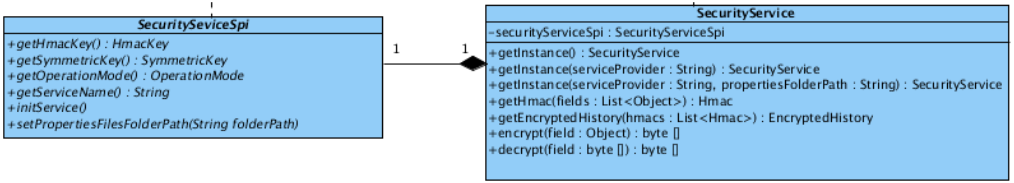
\includegraphics[width=\textwidth]{images/provider.png}
\caption{Representa\c{c}\~{a}o do \textit{provider} da biblioteca} \label{figura:diagramProvider}
\end{center}
\end{figure}

\section{Provider}

\subsection{Remote Callback}

\TODO{uma subseção para isso?}

\section{PKCS\#12 Manager}

\TODO{Ou a seção vai com um nome diferente?}

\section{KeyStore Manager}